\documentclass[polish, twoside, 12pt]{mwart}
\usepackage[polish]{babel}
\usepackage{polski}
\usepackage[T1]{fontenc}
\usepackage[utf8]{inputenc}

\usepackage{hyperref}
\hypersetup{
    colorlinks,
    citecolor=black,
    filecolor=black,
    linkcolor=black,
    urlcolor=black
}
\usepackage{listings}

\usepackage{tikz-qtree}

\usepackage{graphicx}
\graphicspath{ {../figures/} }

\let\stdsection\section
\renewcommand*{\section}{\clearpage\stdsection}
\emergencystretch=3em
\linespread{1.1}

\author{Kewin Polok}
\title{Praca dyplomowa magisterska}

\begin{document}

\maketitle
 
\newpage

\tableofcontents

\newpage

\listoffigures
 
\listoftables

\newpage

\section{Wstęp}

\subsection{Cel pracy}

\subsection{Układ pracy}

\section{Specyfikacja problemu}

\subsection{Założenia dotyczące problemu}

\section{Przeglądarka internetowa}

Przeglądarka internetowa (ang. \emph{web browser}) to program komputerowy służący do pobierania i wyświetlania stron internetowych udostępnianych przez serwery WWW. Komunikacja z serwerem odbywa się najczęściej za pomocą protokołu HTTP (ang. \emph{Hypertext Transfer Protocol})lub odpowiednika w wersji szyfrowanej HTTPS (ang. \emph{Hypertext Transfer Protocol Secure}). Nierzadko przeglądarki internetowe są w stanie obsługiwać inne protokoły takie jak np. FTP (ang. \emph{File Transfer Protocol}) wykorzystywany do serwerów plików, czy też protokoły POP3 (ang. \emph{Post Office Protocol}), IMAP (ang. \emph{Internet Message Access Protocol}) i SMTP (ang. \emph{Simple Mail Transfer Protocol}) wykorzystywane do poczty elektronicznej. 

\begin{figure}[ht]
  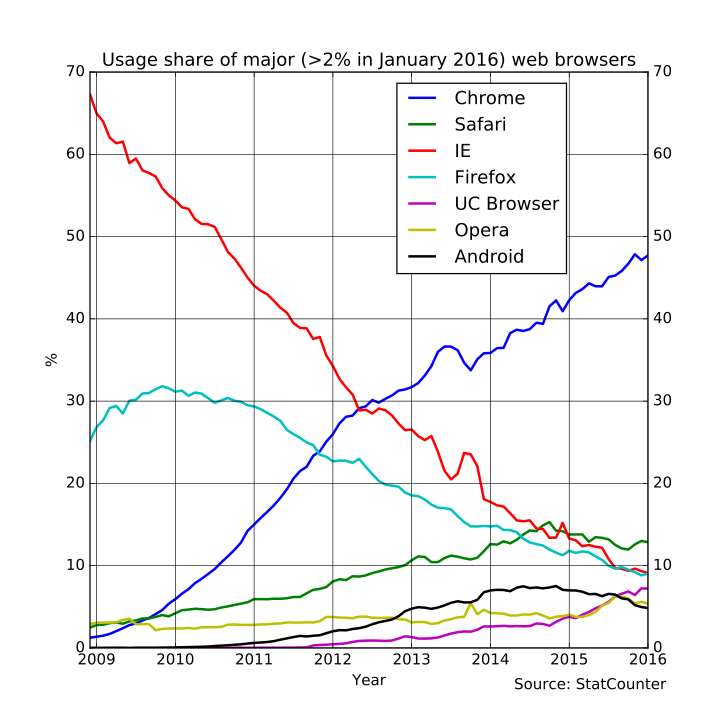
\includegraphics[width=\textwidth]{web-browers-usage-share.png}
	\caption{Udział najwaznieższych przeglądarek na rynku w latach 2009-2016}
\end{figure}

\subsection{Technologie}

Współczesne strony internetowe to nierzadko bardzo skompliowane aplikacje, dlatego też przeglądarki internetowe muszą bardzo dobrze obsługiwać wiele technologii, które działając razem pozwalają dostarczyć bardzo wysokiej jakości doświadczenia użytkownika (ang. \emph{User experience}). 

\subsubsection{HTML 5.1} \label{html}

Hipertekstowy język znaczników (ang. \emph{HyperText Markup Language}) to język służący do określenia struktury strony internetowej. Definicję HTML 5.1 stanowi W3C REC-HTML51 \cite{w3c-rec-html51}. Oprócz głównego tekstu HTML zawiera tak zwane znaczniki, które zawierają dodatkowe informacje pozwalające przeglądarce internetowej odpowiednio zinterpretować określony fragment strony interetowej. Za pomocą znaczników możemy formować fragmenty strony w takie struktury jak hiperłącza, akapity, listy, nagłówki, czy też formularze. Znaczniki najczęściej występują w parach (jako znacznik otwierając oraz zamykający) definiując zakres działania.

\lstinputlisting[language=HTML, caption=Przykładowa prosta strona internetowa z formularzem]{../src/examples/html.html}

Strona internetowa zaczyna się od \emph{<!DOCTYPE html>}. Jest to specjalny znacznik, który musi być umieszczony jako pierwszy. Informuje on przeglądarkę o tym, że tekst jest w formacie HTML. Kolejnym znacznikiem jest \emph{html} z atrybutem \emph{lang}, jest to główny znacznik, będacy korzeniem całej zagnieżdzonej struktury. Dodatkowo informuje o. Bardzo ważny, wyraźnie odseparowany fragment to znacznik \emph{head} zawierający infomację o systemie kodowania (w tym wypadku jest to  kodowanie UTF-8) oraz tytuł strony. Może on zawierać dodatkowe metadane opisujące stronę internetową. Z punktu widzenia użytkownika najważniejszym fragmentem jest znacznik \emph{body}, który zawiera właściwą treść, czyli w tym wypadku jest to głównie formularz \emph{form}. Dwa najważniejsze atrybuty opisujące formularz to \emph{action} informujący przeglądarkę gdzie wysłać dane wpisane przez użytkownika oraz \emph{method} na podstawie, którego przeglądarka wie jaką metodę protokołu HTTP zastosować. Przykładowy formularz zawiera jedno pole tekstowe \emph{input type="text"} oraz jedno pole do wpisywania haseł \emph{input type="password"}. Hasło wpisane w tego typu pole jest domyślnie ukryte przez przeglądarkę dla celów bezpieczeństwa. Oba pola dodatkowo opisane są etykietami \emph{label}. Ostatnim nieopisanym jeszcze znacznikiem jest \emph{button type="submit"}, który jest po prostu przyciskiem służącym do wysłania formularza. Każda przeglądarka posiada wbudowany zestaw styli, który definiuje wygląd każdego znacznika przewidzianego w dokumentacji HTML 5.

\begin{figure}[ht]
  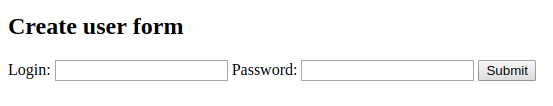
\includegraphics[width=\textwidth]{html-chrome.png}
	\caption{Przykład wyrenderowany w przeglądarce Chrome}
\end{figure}

\subsubsection{CSS 3}

Kaskadowe arkusze stylów (ang. \emph{Cascading Style Sheets}) to język służący do opisu wyświetlania struktury opisanej w języku HTML. Wersja 3 składa się z wielu modułów. Każdy z nich dodaje nowe możliwości lub rozszerza te zdefiniowane w CSS 2 zachowując wsteczną kompatybilność (ang. \emph{backward compatibility}).

\begin{itemize}
  \item css3-background - specyfikacja W3C REC-CSS3-Background \cite{w3c-rec-css3-background}
  \item css3-box - specyfikacja W3C REC-CSS3-Box \cite{w3c-rec-css3-box}
  \item css-cascade-3 - specyfikacja W3C REC-CSS-Cascade-3 \cite{w3c-rec-css3-cascade}
  \item css3-color - specyfikacja W3C REC-CSS3-Color \cite{w3c-rec-css3-color}
  \item css3-content - specyfikacja W3C REC-CSS-Content-3 \cite{w3c-rec-css3-content}
  \item css-fonts-3 - specyfikacja W3C REC-CSS-Fonts-3 \cite{w3c-rec-css3-fonts}
  \item css3-gcpm - specyfikacja W3C REC-CSS-GCPM-3 \cite{w3c-rec-css3-gcpm}
  \item css3-layout - specyfikacja W3C REC-CSS-Template-3 \cite{w3c-rec-css3-template}
  \item css3-mediaqueries - specyfikacja W3C REC-CSS3-Mediaqueries \cite{w3c-rec-css3-mediaqueries}
  \item css3-multicol - specyfikacja W3C REC-CSS3-Multicol \cite{w3c-rec-css3-multicol}
  \item css3-page - specyfikacja W3C REC-CSS3-Page \cite{w3c-rec-css3-page}
  \item css3-selectors - specyfikacja W3C REC-CSS3-Selectors \cite{w3c-rec-css3-selectors}
  \item css-3-ui - W3C REC-CSS-UI-3 \cite{w3c-rec-css3-ui}
\end{itemize}

Za pomocą CSS opisać można wszystkie pojęcia odpowiedzialne za reprezentację elementów HTML, takie jak rodzina czcionek, kolor tekstu, marginesy, czy też pozycja danego elementu względem innych elementów lub okna przeglądarki.

CSS został stworzony w celu odseparowania struktury dokumentu od formy jego prezentacji. Zalety tej separacji to zwiększony zakres dostępności witryny, zmniejszona zawiłość dokumentu, łatwiejsze wprowadzanie zmian w strukturze dokumentu. CSS ułatwia także zmiany w wyświetlaniu strony w zależności od obsługiwanego medium (ekran komputera, ekran tabletu, ekran telefonu komórkowego).

Arkusz stylów składa się z reguł określających styl dla wybranych elementów dokumentu. Reguła składa się z selektora oraz deklaracji. Selektor określa grupę elementów, którego ma dotyczyć deklaracja. Deklaracja określa formatowanie i składa się z nazwy jednej z właściwości i jej wartości napisanej po dwukropku. Deklaracja musi być otoczona nawiasami klamrowymi.

\begin{lstlisting}
selektor { 
	wlasciwosc: wartosc; 
}
\end{lstlisting}

Selektory oraz deklaracje można grupować. Zgrupowane selektory rozdziela się przecinkami, natomiast deklaracje średnikami.

\begin{lstlisting}
selektor, selektor2 { 
	wlasciwosc1: wartosc1;
	wlasciwosc2: wartosc2;
}
\end{lstlisting}

Selektory mogą poszukiwać elementy na podstawie wielu różnych wartośći, jedne z nich to:

\begin{itemize}
  \item nazwa elementu np. \emph{h1}
  \item atrybut \emph{class} elementu np. \emph{.my-class}
  \item identyfikator elementu, czyli atrybut \emph{id} np. \emph{\#element-id}
  \item połączenie wcześniejszych selektorów operatorem logicznym \emph{OR} np. \emph{h1.my-class}
  \item połączenie wcześniejszych selektorów operatorem logicznym \emph{AND} np. \emph{\#element-id .my-class}
\end{itemize}

Dobrą praktyką jest definiowanie selektorów na podstawie atrubutu \emph{class}, natomiast identyfikator, czyli atrybut \emph{id} powinien służyć do jednoznacznej identyfikacji elementu w strukturze HTML. Zgodnie z dokumentacją wiele znaczników może posiadać taką samą klasę, natomiast identyfikator aby spełniał swoje zadanie musi być unikalny.

Ponieważ standardowy wygląd znaczników z punktu widzenia użytkownika może być interpretowany jako bardzo prosty to współcześnie nieostylowane strony internetowe zdarzają się bardzo rzadko. W celu pokazania jak duża może być różnica pomiędzy standardowym, a specjalnie ostylowanym wyglądem strony internetowej przedstawiony zostanie poprzedni przykład strony z formularzem wzbogacony o bardzo lekką bibliotekę CSS o nazwie Milligram\cite{milligram}, której rozmiar wynosi tylko 2kb.

\begin{figure}[ht]
  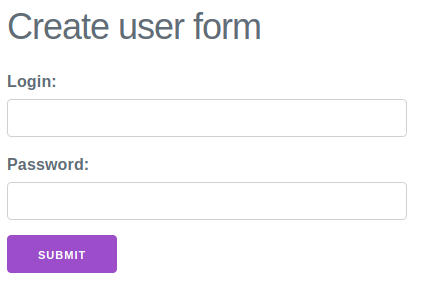
\includegraphics[width=\textwidth]{html-css-chrome.png}
	\caption{Ostylowany przykład wyrenderowany w przeglądarce Chrome}
\end{figure}

\subsubsection{JavaScript}

JavaScript to skryptowy język programowania, stworzony przez firmę Netscape, najczęściej stosowany na stronach internetowych. Pod koniec lat 90. XX wieku organizacja ECMA wydała na podstawie JavaScriptu standard języka skryptowego o nazwie ECMAScript. Najnowsza stabilna wersja ECMAScript nosi nazwę ECMAScript 2016 \cite{es2016} i została wydana 17 czerwca 2016. Organizacja ECMA zapowiedziała, że stabilna wersja tego standardu od wersji 2015 będzie ogłaszana co rok i to właśnie rok wydania będzie jednoznaczny z numerem wersji. Wcześniej mowa była o edycji standardu ECMAScript i do teraz często można się spotkać z zamiennem stosowaniem nazw ECMAScript 6 i ECMAScript 2015 (skracanych odpowiednio do ES6 i ES2015).

Najczęściej spotykanym zastosowaniem języka JavaScript są strony WWW. Skrypty napisane w tym języku najczęściej służą do zapewnienia interaktywności poprzez odpowiednie reagowanie na zdarzenia generowane przez użytkownika. Skrypty JavaScriptu uruchamiane przez strony internetowe mają znacznie ograniczony dostęp do komputera użytkownika. 

Platformy programistyczne, które zostaną zbadane w ramach pracy magisterskiej napisane są języku JavaScript. Wspomagają one proces pisania aplikacji internetowej dostarczając odpowiednich funkcji i organizująć strukturę strony internetowej zgodnie z wytycznymi konkretnej platformy programistycznej.

W języku HTML za umieszczanie skryptów JavaScript odpowiedzialny jest znacznik \emph{script} z opcjonalnymi parametrami \emph{type="text/javascript"} i \emph{language="javascript"}.

JavaScript może zostać użyty również po stronie serwera dzięki darmowemu środowisku uruchomieniowemu Node.js\cite{node.js}. Node.js zaprojektowany został do tworzenia wysoce skalowalnych aplikacji internetowych, szczególnie właśnie serwerów napisanych w języku JavaScript. Architektura Node.js składa się z silnika V8 \cite{v8} stworzonego przez Google i opiera się na sterowaniu zdarzeniami wykorzystującymi asynchroniczny system wejścia-wyjścia. Kod źródłowy jest otwarty (ang. \emph{open source}) i każdy może brać udział w jego rozwijaniu. Domyślnym menedżer pakietów dla Node.js jest Npm \cite{npm}, jednak warto zapoznać się z alternatywnym mendedżerem o nazwie Yarn \cite{yarn}, którego głównymi zaletami są szybsze pobieranie zależności oraz bardziej płaska stuktura drzewa pobranych zależności.

\subsubsection{DOM}

Obiektowy model dokumentu (ang. \emph{Document Object Model}) to zespół klas i interfejsów programistycznych umożliwiających dostęp do elementów strony napisanej w języku HTML. Istnieje kilka tzw. poziomów DOM (ang. \emph{level}):

\begin{itemize}
  \item DOM Level 0 - nie stanowi oficjalnego standardu W3C \cite{w3c}, pierwotnie był modelem zaimplementowanym w przeglądarce Netscape Navigator 3.0, obecnie wspierają go wszystkie przeglądarki
  \item DOM Level 1 - specyfikacja W3C REC-DOM-Level-1 \cite{w3c-rec-dom-level-1} 
  \item DOM Level 2 - specyfikacja W3C REC-DOM-Level-2 \cite{w3c-rec-dom-level-2} 
  \item DOM Level 3 - definicję stanowi sześć specyfikacji
  \begin{itemize}
    \item DOM Level 3 Core - specyfikacja W3C DOM-Level-3-Core \cite{w3c-rec-dom-level-3-core}
    \item DOM Level 3 Load and Save - specyfikacja W3C DOM-Level-3-LS \cite{w3c-rec-dom-level-3-ls}
    \item DOM Level 3 XPath - specyfikacja W3C DOM-Level-3-XPath \cite{w3c-rec-dom-level-3-xpath}
    \item DOM Level 3 Views and Formatting - specyfikacja W3C DOM-Level-3-Views \cite{w3c-rec-dom-level-3-views}
    \item DOM Level 3 Requirements - specyfikacja W3C DOM-Level-3-Requirements \cite{w3c-rec-dom-level-3-requirements}
    \item DOM Level 3 Validation - specyfikacja W3C DOM-Level-3-Val \cite{w3c-rec-dom-level-3-val}
  \end{itemize}
\end{itemize}

DOM pozwala dokonywać dowolnych modyfikacji poprzez tworzenie, usuwanie i modyfikację tzw. węzłów (ang. \emph{nodes}). Początkowo nie istniał standardowy obiektowy model dokumentu. Twórcy najpopulaniejszych przeglądarek tworzyłi własne niezgodne ze sobą modele. Organizacja W3C \cite{w3c} przygotowała ujednolicony standard obiektowego modelu dokumentu, w którym dokment jest dostępny pod postacią globalnego obiektu \emph{document}, który posiada metody do np. pobierania elementu na podstawie identyfikatora \emph{document.getElementById} lub na podstawie klasy \emph{document.getElementByClassName}. Standard W3C definiuje interfejsy DOM tylko dla języków JavaScript i Java.

\begin{figure}
  \centering
  \begin{tikzpicture}
    \Tree[.html 
      [.head 
        [.meta ]
        [.title ]
      ]
      [.body 
        [.h2 ]
        [.form 
            [.label ]
            [.input ]
            [.label ]
            [.input ]
            [.button ]
        ]
      ]
    ]
  \end{tikzpicture}
  \caption{Drzewo DOM wygenerowane dla przykładu opisanego w rozdziale \ref{html}}
\end{figure}

\subsubsection{HTTP/1.1}

Protokół przesyłania dokumentów hipertekstowych (ang.\emph{(Hypertext Transfer Protocol)}) to protokół za pomocą którego przysła się żadania udostępnienia dokumentów z serwera WWW oraz informacje z forumlarzy internetowych. Obecną definicję HTTP stanowi RFC 2616 \cite{rfc2616}

Protokół HTTP udostępnia znormalizowany sposób komunikowania się komputerów ze sobą. Określa on formę żądań (ang. \emph{requests}) klienta dotyczących danych oraz formę odpowiedzi (ang. \emph{responses}) serwera na te żądania. Klientem może być np. przeglądarka internetowa. Jest zaliczany do protokołów bezstanowych (ang. \emph{stateless}) ponieważ nie zachowuje żadnych informacji o poprzednich transakcjach z klientem. Pozwala to znacznie zmniejszyć obciążenie serwera, jednak uniemożliwia zapamiętanie konkretnego stanu użytkownika w sytuacji gdy jest to potrzbne np. przy implementacji koszyka z zakupami w sklepie internetowym. Najczęstszym rozwiązaniem tego problemu jest wprowadzenie mechanizmu ciasteczek (ang. \emph{cookies}). Ciasteczka to mały fragment tekstu zawierający pary klucz-wartość. Przesyłane są one z każdym żądaniem do serwera. Alternatywne rozwiązania to ukryte parametry (gdy aktualna strona zawiera formularz) oraz parametry umieszczone w ujednoliconym formacie adresowania zasobów (ang. \emph{Uniform Resource Locator}.

Wywołania protokołu HTTP zaczynają się od \url{http://}. HTTP standardowo korzysta z portu numer 80 protokołu kontroli transmisji (ang. \emph{Transmission Control Protocol}).

Zapytanie HTTP zaczynaja się od nazwy metody, która określa akcję jaką obiekt tworzący zapytanie chce wykonać na zasobie podstępnym pod określonym adresem. Dostępne metody to:

\begin{enumerate}
  \item \emph{GET} - pobranie zasobu
  \item \emph{HEAD} - pobranie informacji o zasobie, metoda stosowana do sprawdzania dostępności zasobu
  \item \emph{PUT} - aktualizacja zasobu
  \item \emph{POST} - stworzenie nowego zasobu
  \item \emph{DELETE} - usunięcie zasobu
  \item \emph{OPTIONS} - pobranie informacji o możliwych operacjach do wykonania na zasobie
  \item \emph{TRACE} - metoda stosowana do diagnostyki kanału komunikacyjnego
  \item \emph{PATCH} - częściowa aktualizacja zasobu
\end{enumerate}

Poniżej przedstawione przykładowe żądanie HTTP/1.1 przeglądarki Chrome i odpowiedź serwera opisanego w rozdziale \ref{server}.

\begin{lstlisting}[caption=Przykładowe żądanie HTTP/1.1,]
GET / HTTP/1.1
Host: localhost:8080
Connection: keep-alive
Pragma: no-cache
Cache-Control: no-cache
Upgrade-Insecure-Requests: 1
User-Agent: Mozilla/5.0 (X11; Linux x86_64) AppleWebKit/537.36 
  (KHTML, like Gecko) Chrome/60.0.3112.90 Safari/537.36
Accept: text/html,application/xhtml+xml,application/xml;q=0.9,
  image/webp,image/apng,*/*;q=0.8
Accept-Encoding: gzip, deflate, br
Accept-Language: pl-PL,pl;q=0.8,en-US;q=0.6,en;q=0.4
\end{lstlisting}

\begin{lstlisting}[caption=Przykładowa odpowiedź HTTP/1.1]
HTTP/1.1 200 OK
X-Powered-By: Express
Content-Type: text/html; charset=utf-8
Content-Length: 116
ETag: W/"74-IGpXmXtcB0E/yn+QbK3UFXMrMU8"
Date: Tue, 15 Aug 2017 10:28:41 GMT
Connection: keep-alive
\end{lstlisting}

\subsubsection{HTTPS}

Bezpieczny protokół przesyłania dokumentów hipertekstowych (ang. \emph{Hypertext Transfer Protocol Secure}) to szyfrowana wersja protokołu HTTP. Obecną definicję HTTPS stanowi RFC 2660 \cite{rfc2660}

W odróżnieniu od protokołu HTTPS protokół HTTP do komunikacji stosuje niezaszyfrowany tekst. HTTPS początkowo szyfrował dane za pomocą protokołu SSL (ang. \emph{Secure Socket Layer}), natomiast obecnie używany jest protokół TLS (ang. \emph{Transport Layer Security}). Szyfrowanie zapobiega przechtywywaniu i zmienianiu przesyłanych danych. 

Wywołania protokołu HTTPS zaczynają się od \url{https://}. HTTPS standardowo korzysta z portu numer 443 protokołu kontroli transmisji. 

\subsubsection{HTTP/2}

Protokół HTTP/2 to unowocześniejszego protokołu HTTP/1.1. Został on opracowany na podstawie wczesnych wersji ekperymentalnego protokołu SPDY \cite{spdy}. Obecną definicję HTTP/2 stanowi RFC 7540 \cite{rfc7540}. Poniżej przedstawiono najważniejsze zalety protokołu HTTP/2

\begin{enumerate}
  \item \emph{Multipleksowanie} - protokół nawiązuje tylko jedno trwałe połączenie z serwerem za pomocą którego pobierane są wszystkie pliku niezbędne do prawidłowego wyświetlenia strony
  \item \emph{Powiadomienia Push} - serwer może wysłać dodatkowe informacje np. może wysłać pliki, które są potrzebne do prawidłowego wyświetlenia strony zanim przeglądarka internetowa zauważy tą potrzebę
  \item \emph{Ustalanie priorytetów} - każde zapytanie o plik posiada swój priorytet, który nadawany jest przez serwer. Umożliwia to najpierw pobranie najważniejszych plików, które pozwolą wyrenderować kluczowe fragmenty strony internetowej, a następnie doczytać kolejne elementy
  \item \emph{Kompresja nagłówków} - protokół HTTP/2 unika duplikacji informacji występującyh pomiędzy różnymi nagłówkami i wysyła je w skompresowanym formacie
  \item \emph{Szyfrowanie} - pomimo, iż szyfrowanie według protokołu HTTP/2 nie jest wymagane to większość najważniejszych przeglądarek internetowych implementuje HTTP/2 wyłącznie z wykorzystaniem protokołu TLS
\end{enumerate}

\begin{figure}[ht]
  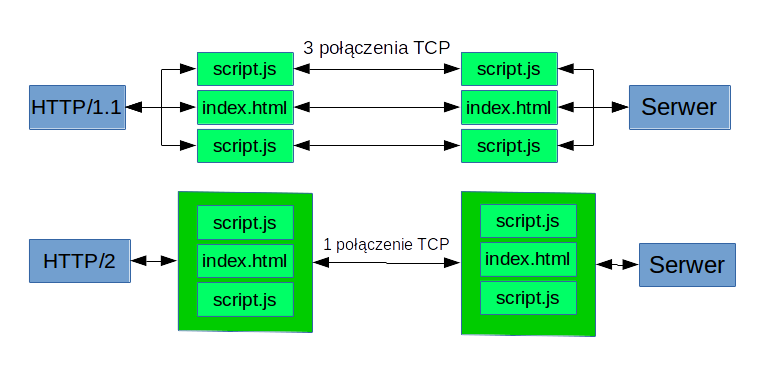
\includegraphics[width=\textwidth]{http2-mux.png}
	\caption{Multipeksowanie HTTP/2}
\end{figure}

\subsection{Mechanizm ładowania strony internetowej i jej zasobów}

\subsection{Model współbieżności oraz pętla zdarzeń}

\section{Aplikacja do badań wydajnościowych i czasowych}

\section{Serwer dla aplikacji internetowych} \label{server}

\subsubsection{Opis}

\subsubsection{Implementacja}

\subsubsection{Komponenty}

\section{Biblioteki programistyczne do tworzenia aplikacji internetowyuch}

\subsection{Cechy}

\subsection{Porównanie}

\subsection{Angular 1}

\subsubsection{Opis}

\subsubsection{Wady i zalety}

\subsubsection{Mechanizm działania}

\subsubsection{Implementacja}

\subsection{Angular 2}

\subsubsection{Opis}

\subsubsection{Wady i zalety}

\subsubsection{Mechanizm działania}

\subsubsection{Implementacja}

\subsection{React}

\subsubsection{Opis}

\subsubsection{Wady i zalety}

\subsubsection{Mechanizm działania}

\subsubsection{Implementacja}

\subsection{Vue.js}

\subsubsection{Opis}

\subsubsection{Wady i zalety}

\subsubsection{Mechanizm działania}

\subsubsection{Implementacja}

\subsection{Mithril.js}

\subsubsection{Opis}

\subsubsection{Wady i zalety}

\subsubsection{Mechanizm działania}

\subsubsection{Implementacja}

\section{Badania wydajnościowe}

\subsection{Badania wydajności pamięciowej}

\subsection{Badania wydajności czasowej}

\section{Porównanie wyników i wnioski}

\section{Podsumowanie}

\subsection{Dalszy rozwój}

\begin{thebibliography}{11}
  \bibitem{milligram}
    \url{http://milligram.io/}
  \bibitem{node.js}
    \url{http://nodejs.org/}
  \bibitem{v8}
    \url{https://github.com/v8/v8}
  \bibitem{npm}
    \url{https://www.npmjs.com/}
  \bibitem{yarn}
    \url{https://yarnpkg.com/}
  \bibitem{es2016}
    \url{https://www.ecma-international.org/ecma-262/7.0/}
  \bibitem{spdy}
    \url{http://dev.chromium.org/spdy/}
  \bibitem{w3c}
    \url{https://www.w3.org/}
  \bibitem{w3c-rec-html51}
    \url{https://www.w3.org/TR/html51/}
  \bibitem{w3c-rec-css3-background}
    \url{https://www.w3.org/TR/css3-background/}
  \bibitem{w3c-rec-css3-box}
    \url{https://www.w3.org/TR/css3-box/}
  \bibitem{w3c-rec-css3-cascade}
    \url{https://www.w3.org/TR/css-cascade-3/}
  \bibitem{w3c-rec-css3-color}
    \url{https://www.w3.org/TR/css3-color/}
  \bibitem{w3c-rec-css3-content}
    \url{https://www.w3.org/TR/css-content-3/}
  \bibitem{w3c-rec-css3-fonts}
    \url{https://www.w3.org/TR/css-fonts-3/}
  \bibitem{w3c-rec-css3-gcpm}
    \url{https://www.w3.org/TR/css-gcpm-3/}
  \bibitem{w3c-rec-css3-template}
    \url{https://www.w3.org/TR/css-template-3/}
  \bibitem{w3c-rec-css3-mediaqueries}
    \url{https://www.w3.org/TR/css3-mediaqueries/}
  \bibitem{w3c-rec-css3-multicol}
    \url{https://www.w3.org/TR/css3-multicol/}
  \bibitem{w3c-rec-css3-page}
    \url{https://www.w3.org/TR/css3-page/}
  \bibitem{w3c-rec-css3-selectors}
    \url{https://www.w3.org/TR/css3-selectors/}
  \bibitem{w3c-rec-css3-ui}
    \url{https://www.w3.org/TR/css-ui-3/}
  \bibitem{w3c-rec-dom-level-1}
    \url{https://www.w3.org/TR/DOM-Level-1/}
  \bibitem{w3c-rec-dom-level-2}
    \url{https://www.w3.org/TR/DOM-Level-2/}
  \bibitem{w3c-rec-dom-level-3-core}
    \url{https://www.w3.org/TR/DOM-Level-3-Core/}
  \bibitem{w3c-rec-dom-level-3-ls}
    \url{https://www.w3.org/TR/DOM-Level-3-LS/}
  \bibitem{w3c-rec-dom-level-3-xpath}
    \url{https://www.w3.org/TR/DOM-Level-3-XPath/}
  \bibitem{w3c-rec-dom-level-3-views}
    \url{https://www.w3.org/TR/DOM-Level-3-Views/}
  \bibitem{w3c-rec-dom-level-3-requirements}
    \url{https://www.w3.org/TR/DOM-Requirements/}
  \bibitem{w3c-rec-dom-level-3-val}
    \url{https://www.w3.org/TR/DOM-Level-3-Val/}
  \bibitem{rfc2616}
    \url{https://www.ietf.org/rfc/rfc2616}
  \bibitem{rfc2660}
    \url{https://www.ietf.org/rfc/rfc2660}
  \bibitem{rfc7540}
    \url{https://www.ietf.org/rfc/rfc7540}
\end{thebibliography}

\end{document}
